\documentclass[%
paper=a4,						% alle weiteren Papierformat einstellbar
%landscape,						% Querformat
fontsize=11pt,					% Schriftgröße (12pt, 11pt (Standard))
%BCOR1cm,						% Bindekorrektur, bspw. 1 cm
DIV=calc,						% führt die Satzspiegelberechnung neu aus
								% s. scrguide 2.4
%twoside,						% Doppelseiten
%twocolumn,						% zweispaltiger Satz
parskip=half,					% Absatzformatierung s. scrguide 3.1
%headsepline,					% Trennline zum Seitenkopf	
%footsepline,					% Trennline zum Seitenfuß
titlepage,						% Titelei auf eigener Seite
headings=big,				% Überschriften etwas kleiner (smallheadings)
%idxtotoc,						% Index im Inhaltsverzeichnis
%liststotoc,					% Abb.- und Tab.verzeichnis im Inhalt
bibliography=totoc,				% Literaturverzeichnis im Inhalt
%abstracton,					% Überschrift über der Zusammenfassungan	
%leqno,   						% Nummerierung von Gleichungen links
%fleqn,							% Ausgabe von Gleichungen linksbündig
%draft							% überlangen Zeilen in Ausgabe gekennzeichnet
]
{scrartcl}

\usepackage[pdftex]{graphicx} 
\usepackage[ngerman]{babel}	
\usepackage[utf8]{inputenc}		
\usepackage[T1]{fontenc}								
\usepackage{lmodern}
\usepackage{color}
\usepackage{booktabs}
\usepackage{array}

% Links im PDF
\usepackage{hyperref}
\definecolor{LinkColor}{rgb}{0,0,0.5}
\hypersetup{
	colorlinks=true,
	linkcolor=LinkColor,
	citecolor=LinkColor,
	filecolor=LinkColor,
	menucolor=LinkColor,
	urlcolor=LinkColor}
	
%Kopf u. Fußzeilen
\usepackage{scrpage2}
\pagestyle{scrheadings}
\clearscrheadfoot
%\chead{}
%\ofoot{}
\cfoot{\pagemark}

\usepackage{mdwlist}
\usepackage{csquotes}

% Neues bibliographie paket
% style=apa
\usepackage[isbn=false,url=false, doi=false, backend=biber, style=numeric]{biblatex}
%\DeclareLanguageMapping{american}{american-apa}

\usepackage{pdfpages}

\def \varpressetext {<Pressetext angeben>}
\newcommand{\pressetext}[1]{\def \varpressetext {#1}}

\def \vargruppe {<Gruppennummer angeben>}
\newcommand{\gruppe}[1]{\def \vargruppe {#1}}

\def \varmitglieder {<Gruppenmitglieder angeben>}
\newcommand{\mitglieder}[1]{\def \varmitglieder {#1}}

\KOMAoptions{DIV=last}


\pressetext{Programmierparadigmen}
\gruppe{9}
\mitglieder{Markus Kirchner}

\begin{document} 

%!TEX root = bewertung-5.tex

\begin{titlepage}
\sffamily

{ \Large Forschungsmethoden WS 2012} \\[2cm]
    
{ \Huge \centering \bfseries Übung 4: Studienzusammenfassung \\[1.5cm] }

{ \LARGE \centering \bfseries \varpressetext \\[1.5cm] }

{
    \begin{flushright}
    { \large
       { \bfseries Bewertete Gruppe:~\vargruppe \\ }
       \varmitglieder
    }

    \end{flushright}
}

\vfill

{ \large
   { \bfseries Bewertende Gruppe: 8 \\ }
   Bernhard Fleck \\
   Rafael Konik \\
   Stephan Matiasch \\
   Harald Watzke \\
}
\end{titlepage}


\includepdf[pages=-]{fragebogen-\vargruppe}

\section{Auswertung von \enquote{\varpressetext}}

Eine Aufschlüsselung der Bewertungsskala des Fragebogens welche fortan für die
Kodierung der angekreuzten Antworten verwendet wird ist
Tabelle~\ref{tab:skala} zu entnehmen.

\begin{table}[!ht]
    \caption{Aufschlüsselung der Bewertungsskala}
    \label{tab:skala}
    \begin{center}
        \begin{tabular}{lc}
        \toprule
        \textbf{Bezeichnung} & \textbf{Skalenwert} \\
        \midrule
        Trifft zu & 1 \\
        Trifft eher zu & 2 \\
        Weder noch & 3 \\
        Trifft eher nicht zu & 4 \\
        Trifft nicht zu & 5 \\
        \bottomrule
        \end{tabular}
    \end{center}
\end{table}

\subsection{Auswertung der allgemeinen \enquote{meta}-Bewertung}

Die folgenden Aussagen lassen sich aufgrund der Bewertung treffen:

\begin{itemize}
    \item der Pressetext hat eher gut gefallen
    \item der Pressetext ist eher gut geschrieben
    \item der Pressetext enthält ein paar ungeklärte Begriffe
    \item der Pressetext ist eher nützlich
    \item der \emph{Unique Selling Point} konnte eher gut dargelegt werden
    \item der Pressetext ist eher gut geschrieben
    \item das Thema des Pressetextes ist eher interessant
    \item die Problemstellung wurde eher gut dargelegt
\end{itemize}

\begin{table}[!ht]
    \begin{center}
        \begin{tabular}{lcc}
        \toprule
        \textbf{Aussage} & \textbf{kodierte Antworten} & \textbf{Median} \\
        \midrule
        Der Artikel hat mir gut gefallen & 5, 3, 2 & 3 \\
        Der Artikel ist gut verständlich & 5, 3, 1 & 3 \\
        Der Artikel enthält viele unerklärte Begriffe & 2, 4, 5 & 4 \\
        Der Artikel ist nützlich & 4, 3, 3 & 3 \\
        Der \emph{Unique Selling Point} wurde gut dargelegt & 4, 4, 4 & 4 \\
        Der Artikel ist gut geschrieben & 5, 4, 2 & 4 \\
        Das Thema des Artikels ist interessant & 2, 3, 2 & 2 \\
        Die Problemstellung wird gut dargelegt & 4, 3, 3 & 3 \\
        \bottomrule
        \end{tabular}
    \end{center}
\end{table}

Invertiert man die einzige negative Aussage \enquote{\emph{Der Artikel enthält
viele unerklärte Begriffe}} und mittelt über alle Aussagen hinweg, erhält man,
unter Verwendung der Skala: \enquote{gut gefallen}, \enquote{eher gut
gefallen}, \enquote{weder noch}, \enquote{eher nicht gefallen} und
\enquote{nicht gefallen}, den folgenden Median: 3.
Der Pressetext hat also insgesamt nur einen durchschnittlichen Eindruck hinterlassen, 
weder besonders positiv noch besonders negativ.

Die Übereinstimmung der Probanden untereinander was die Bewertung des
allgemeinen Teils angeht kann als \emph{eher schlecht} bezeichnet werden.
Besonders bei den Fragen {\emph{Der Artikel hat mir gut gefallen}},{\emph{Der Artikel ist gut verständlich}},
 {\emph{Der Artikel enthält viele ungeklärte Begriffe}} und {\emph{Der Artikel ist gut geschrieben}} 
gehen die Meinungen sehr weit auseinander.


\subsection{Auswertung zum Verständnis des Inhaltes}

\begin{table}[!ht]
    \begin{center}
        \begin{tabular}{p{8cm}cc}
        \toprule
        \textbf{Aussage} & \textbf{kodierte Antworten} & \textbf{Median} \\
        \midrule
       Programmierparadigmen sind Vorschriften nach denen entwickelt werden muss & 5, 5, 1 & 5\\
        \addlinespace
        Die Verwendung des generischen Paradigmas erhöht den Testaufwand & 1, 1, 5 & 1 \\
        \bottomrule
        \end{tabular}
    \end{center}
\end{table}

Die Auswertung zeigt, dass der Inhalt des Pressetextes von zwei von drei Probanden
\enquote{gut verstanden} wurde. Die Übereinstimmung der Probanden
untereinander was die Bewertung des inhaltlichen Teils angeht kann als
\emph{durchschnittlich} bezeichnet werden. Es ist interessant, dass zwei der 
drei Probanden die Fragen gleich beantwortet haben, der dritte Proband die Frage jeweils
ganz am anderen Ende der Skala beantwortete.

\documentclass[%
paper=a4,						% alle weiteren Papierformat einstellbar
%landscape,						% Querformat
fontsize=11pt,					% Schriftgröße (12pt, 11pt (Standard))
%BCOR1cm,						% Bindekorrektur, bspw. 1 cm
DIV=calc,						% führt die Satzspiegelberechnung neu aus
								% s. scrguide 2.4
%twoside,						% Doppelseiten
%twocolumn,						% zweispaltiger Satz
parskip=half,					% Absatzformatierung s. scrguide 3.1
%headsepline,					% Trennline zum Seitenkopf	
%footsepline,					% Trennline zum Seitenfuß
titlepage,						% Titelei auf eigener Seite
headings=big,				% Überschriften etwas kleiner (smallheadings)
%idxtotoc,						% Index im Inhaltsverzeichnis
%liststotoc,					% Abb.- und Tab.verzeichnis im Inhalt
bibliography=totoc,				% Literaturverzeichnis im Inhalt
%abstracton,					% Überschrift über der Zusammenfassungan	
%leqno,   						% Nummerierung von Gleichungen links
%fleqn,							% Ausgabe von Gleichungen linksbündig
%draft							% überlangen Zeilen in Ausgabe gekennzeichnet
]
{scrartcl}

\usepackage[pdftex]{graphicx} 
\usepackage[ngerman]{babel}	
\usepackage[utf8]{inputenc}		
\usepackage[T1]{fontenc}								
\usepackage{lmodern}
\usepackage{color}
\usepackage{booktabs}
\usepackage{array}

% Links im PDF
\usepackage{hyperref}
\definecolor{LinkColor}{rgb}{0,0,0.5}
\hypersetup{
	colorlinks=true,
	linkcolor=LinkColor,
	citecolor=LinkColor,
	filecolor=LinkColor,
	menucolor=LinkColor,
	urlcolor=LinkColor}
	
%Kopf u. Fußzeilen
\usepackage{scrpage2}
\pagestyle{scrheadings}
\clearscrheadfoot
%\chead{}
%\ofoot{}
\cfoot{\pagemark}

\usepackage{mdwlist}
\usepackage{csquotes}

% Neues bibliographie paket
% style=apa
\usepackage[isbn=false,url=false, doi=false, backend=biber, style=numeric]{biblatex}
%\DeclareLanguageMapping{american}{american-apa}

\usepackage{pdfpages}

\def \varpressetext {<Pressetext angeben>}
\newcommand{\pressetext}[1]{\def \varpressetext {#1}}

\def \vargruppe {<Gruppennummer angeben>}
\newcommand{\gruppe}[1]{\def \vargruppe {#1}}

\def \varmitglieder {<Gruppenmitglieder angeben>}
\newcommand{\mitglieder}[1]{\def \varmitglieder {#1}}

\KOMAoptions{DIV=last}


\begin{document} 

\begin{titlepage}
\sffamily

{ \Large Forschungsmethoden WS 2012} \\[2cm]
    
{ \Huge \centering \bfseries Übung 4: Gesamt-Studienzusammenfassung \\[1.5cm] }

%{ \LARGE \centering \bfseries \varpressetext \\[1.5cm] }

%{
%    \begin{flushright}
%    { \large
%       { \bfseries Bewertete Gruppe:~\vargruppe \\ }
%       \varmitglieder
%    }
%
%    \end{flushright}
%}

\vfill

{ \large
   { \bfseries Gruppe: 8 \\ }
   Bernhard Fleck \\
   Rafael Konik \\
   Stephan Matiasch \\
   Harald Watzke \\
}
\end{titlepage}


\section{Gesamtzusammenfassung aller Studien} % (fold)
\label{sec:zusammenfassung_aller_studien}

Wie in Abbildung 1 zu erkennen ist gefielen die Pressetexte von Gruppe 4 und 6 am besten. Bei den Artikeln schnitten Gruppen 2 und 3 am besten ab. Positiv fiel auch Gruppe 4 auf. Negativ fielen bei Gruppe 9 und 10 Rechtschreibung und Grammatik und Schreibstil auf, die dem Standard eines Technischen Artikels und einer Universitätslehrveranstaltung bei weitem nicht gerecht waren.

\begin{figure}[h!tbp]
    \begin{center}
        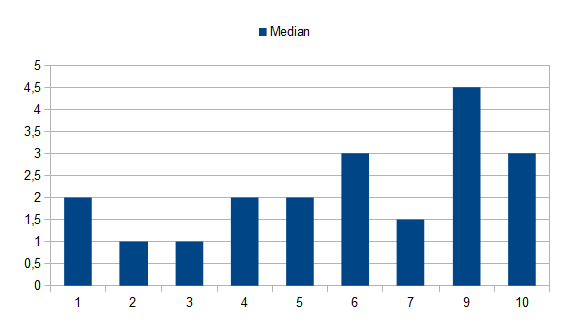
\includegraphics[width=\textwidth]{images/papers_median}
    \end{center}
    \caption{Mediane der Artikel. Die Zahlen 
    stehen von 1 bis 5 für: \enquote{gut gefallen}, \enquote{eher gut 
    gefallen}, \enquote{weder noch}, \enquote{eher nicht gefallen} und 
    \enquote{nicht gefallen}}
    \label{fig:mediane}
\end{figure}

\begin{figure}[h!tbp]
    \begin{center}
        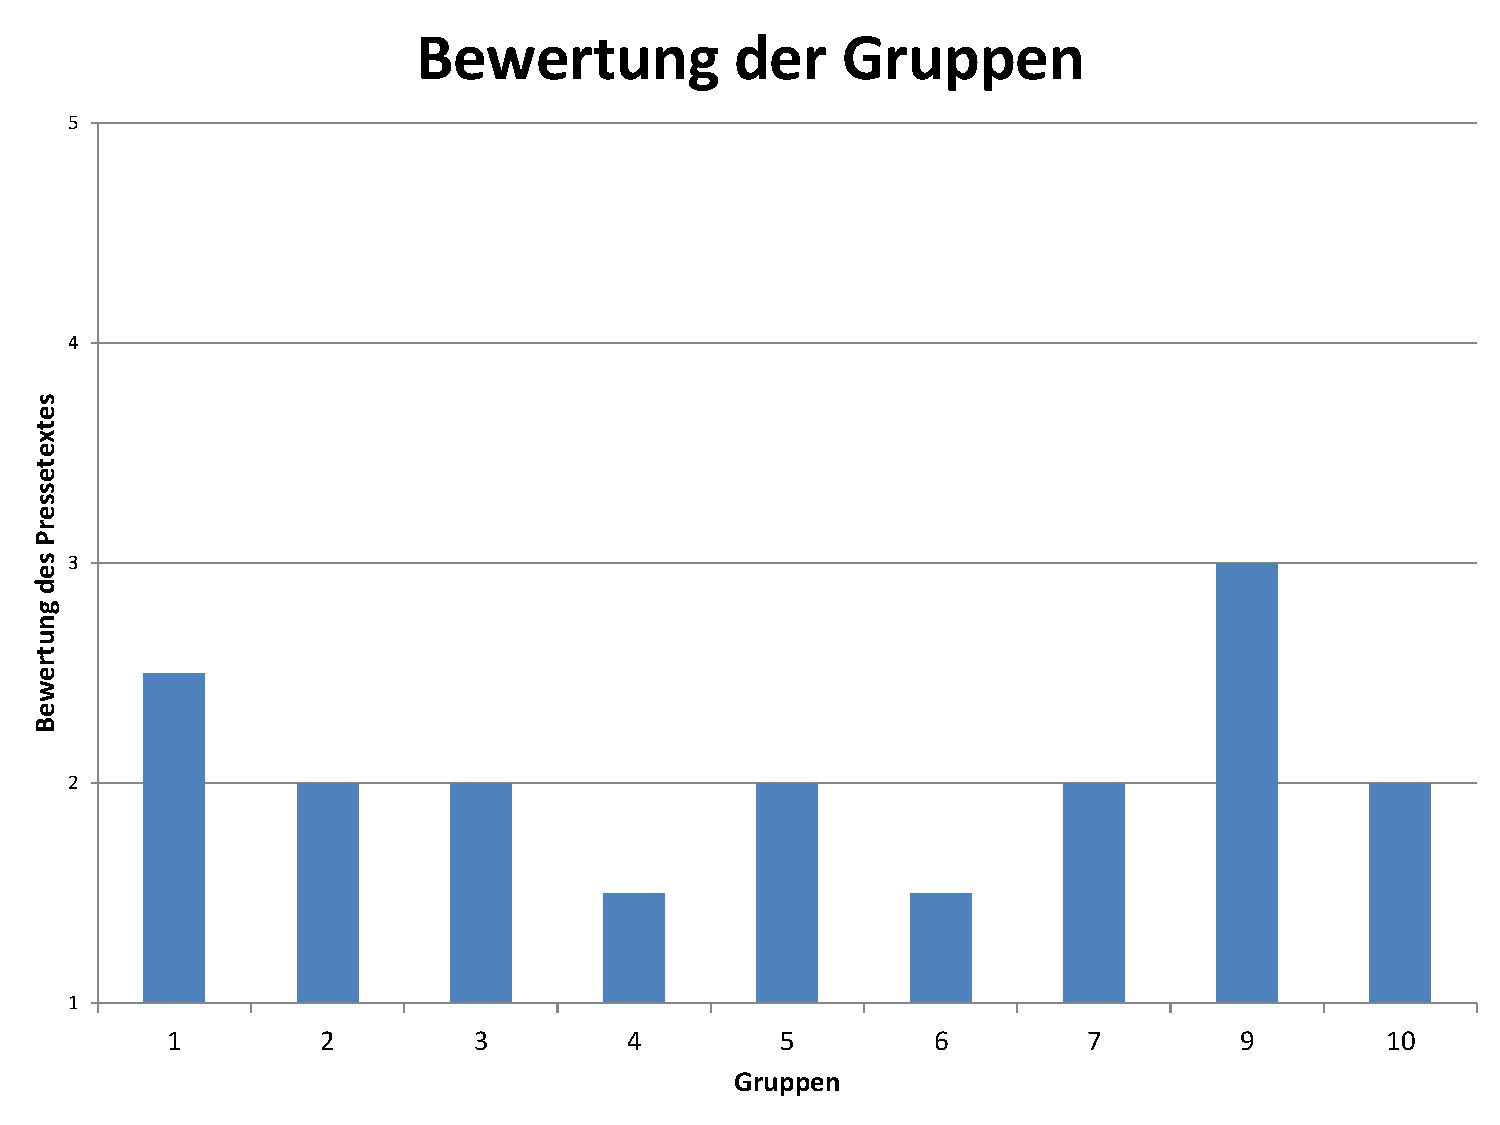
\includegraphics[width=\textwidth]{images/bewertungen}
    \end{center}
    \caption{Bewertung der Pressetexte. Die Zahlen 
    stehen von 1 bis 5 für: \enquote{gut gefallen}, \enquote{eher gut 
    gefallen}, \enquote{weder noch}, \enquote{eher nicht gefallen} und 
    \enquote{nicht gefallen}}
    \label{fig:bewertungen}
\end{figure}

\begin{figure}[h!tbp]
    \begin{center}
        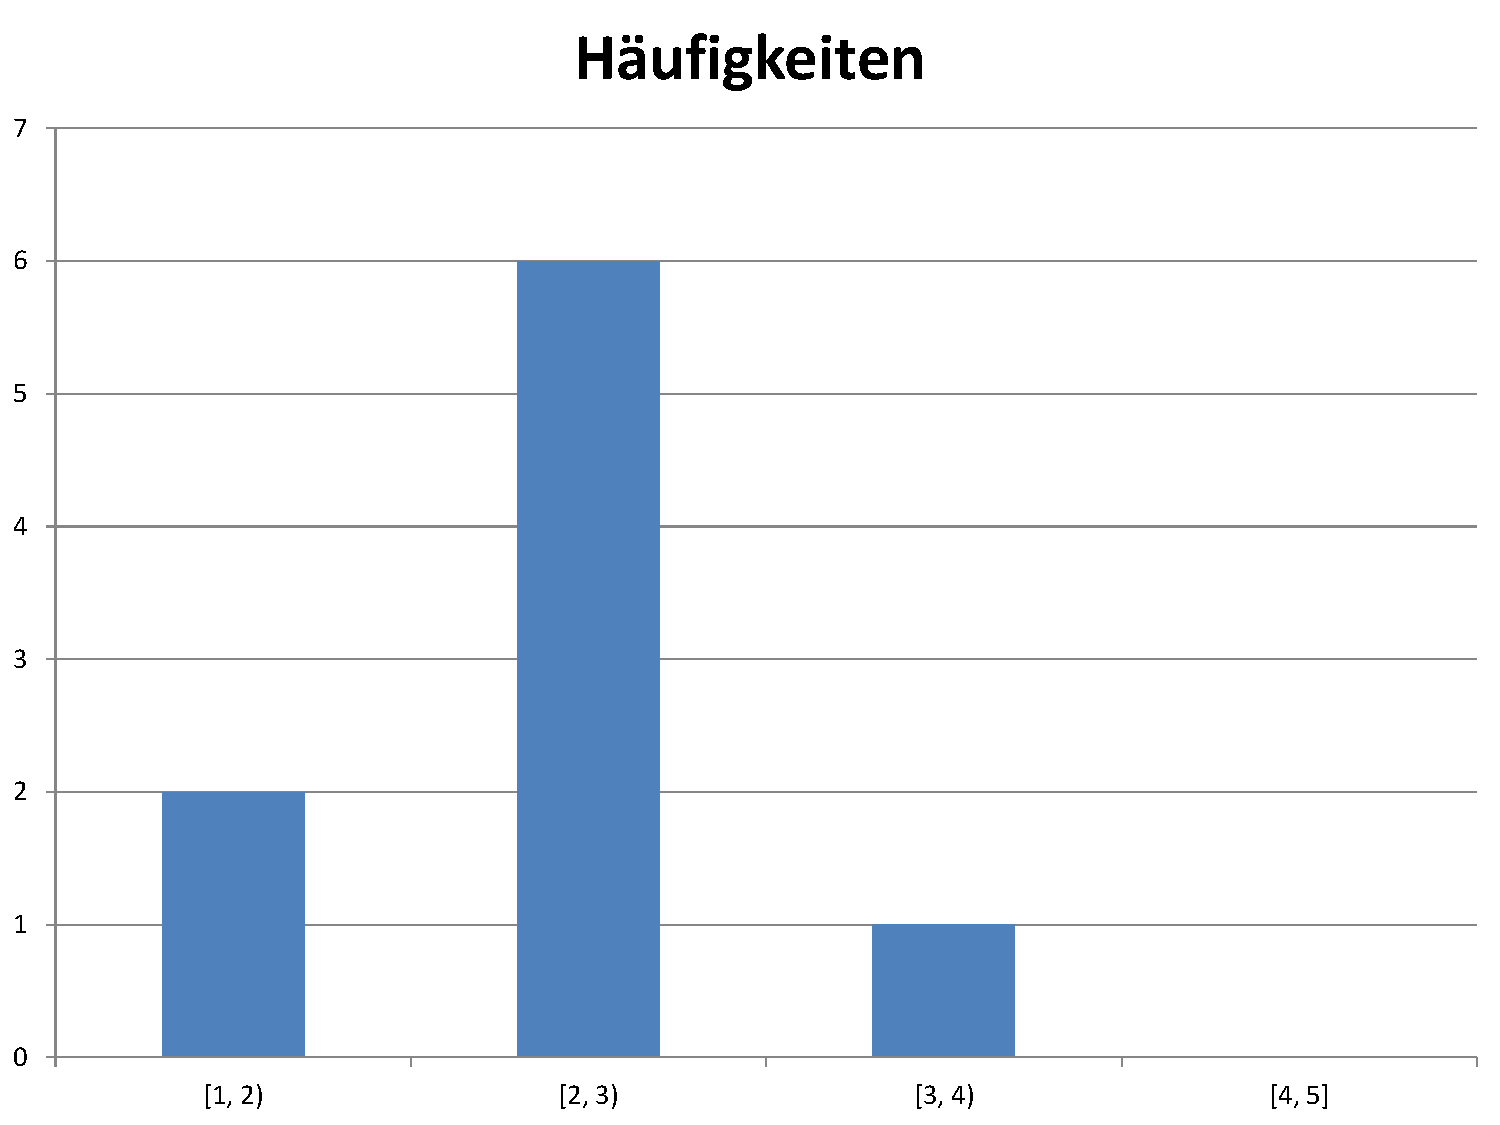
\includegraphics[width=\textwidth]{images/haeufigkeiten}
    \end{center}
    \caption{Häufigkeiten der Bewertungen. Die Zahlen 
    stehen von 1 bis 5 für: \enquote{gut gefallen}, \enquote{eher gut 
    gefallen}, \enquote{weder noch}, \enquote{eher nicht gefallen} und 
    \enquote{nicht gefallen}}
    \label{fig:haeufigkeiten}
\end{figure}

% section zusammenfassung_aller_studien (end)

\end{document}

\includepdf[pages=-]{bewertungen/bewertung_\vargruppe_hw}
\includepdf[pages=-]{bewertungen/bewertung_\vargruppe_rk}
\includepdf[pages=-]{bewertungen/bewertung_\vargruppe_bf}

\end{document}
